% !TEX TS-program = pdfLaTeX+shellescape
% !TEX encoding = UTF-8 Unicode

\documentclass{standalone}
\usepackage{pgfplots}
\pgfplotsset{compat=1.17}

\definecolor{tab_blue}{HTML}{1F77B4}
\definecolor{tab_orange}{HTML}{FF7F0E}
\definecolor{tab_green}{HTML}{2CA02C}
\definecolor{tab_red}{HTML}{D62728}

\begin{document}
    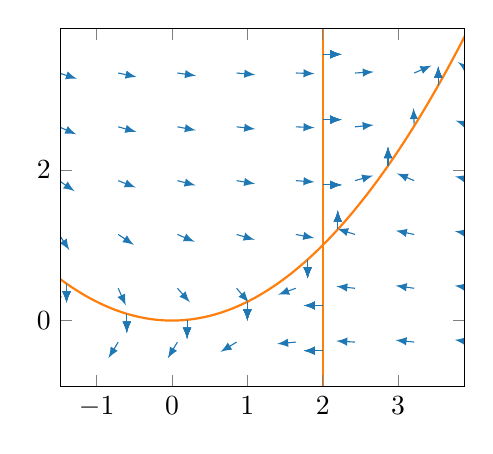
\begin{tikzpicture}[
        baseline,
        declare function = {
            f1(\x, \y) = \y - \x^2; 
            f2(\x, \y) = \x - 2;
            solx(\a,\b,\x) = \a*exp(-\x) + \b*exp(\x);
            soly(\a,\b,\x) = \b*exp(\x);
            derx(\a,\b,\x) = -\a*exp(-\x) + \b*exp(\x);
            dery(\a,\b,\x) = \b*exp(\x);
        }
        ]
        \begin{axis}[
            scale=.8,
            view = {0}{90},
            xmin=-1.48,xmax=3.88,ymin=-0.88,ymax=3.88, % range of plot
            % legend style={at={(axis cs: 1,0)}, anchor=south east}, % position of legends
            unit vector ratio = {1, 1, 1}, % aspect ratio
            % axis lines = box, % middle or box
            %axis x line = bottom, % top, middle, bottom, none: axis x line* = ... removes arrow heads
            %axis y line = left, % left, center, right, none: axis y line* = ... removes arrow heads
            %xlabel = {$x$}, ylabel = {$y$}, % axis labels 
        ]
            \addplot3[tab_blue, quiver={u={(4*y - x^2) / sqrt(16*y^2 - 8*y*x^2 + x^4 + x^2 - 4*x + 4)}, v={(x-2) / sqrt(16*y^2 - 8*y*x^2 + x^4 + x^2 - 4*x + 4)}, scale arrows = 0.25}, domain=-1.5:4.0, y domain=-1.0:4.0, samples=8, -latex] (x, y, 0);
            \addplot3[thick, tab_orange, domain=-2:4, samples=100, samples y=1]({x}, {x^2/4}, {0});
            \addplot3[thick, tab_orange, domain=-1:10, samples=100, samples y=1]({2}, {x}, {0});
            \addplot3[tab_blue, variable=\t, samples=6, domain=-2.2:1.8, -latex, quiver={u={0}, v={-1}, scale arrows=0.25}]({t}, {t^2/4}, {0});
            \addplot3[tab_blue, variable=\t, samples=4, domain=2.2:4.2, -latex, quiver={u={0}, v={1}, scale arrows=0.25}]({t}, {t^2/4}, {0});
            \addplot3[tab_blue, variable=\t, samples=3, domain=-1.0:0.2, -latex, quiver={u={-1}, v={0}, scale arrows=0.25}]({2}, {t}, {0});
            \addplot3[tab_blue, variable=\t, samples=4, domain=1.8:4.4, -latex, quiver={u={1}, v={0}, scale arrows=0.25}]({2}, {t}, {0});
        \end{axis}
    \end{tikzpicture}
\end{document}